\documentclass[12pt,a4paper]{article}
\usepackage[utf8]{inputenc}
\usepackage[T1]{fontenc}
\usepackage[english]{babel}
\usepackage{lmodern}
\usepackage[a4paper,margin=3cm]{geometry}
\usepackage{graphicx}
\usepackage{subcaption}
\usepackage{booktabs}
\usepackage{amsmath}
\usepackage{float}
\usepackage{enumitem}
\usepackage{fancyhdr}
\usepackage{xcolor}
\usepackage{tocloft}
\setlength{\cftbeforesecskip}{0.2em}
\setlength{\cftbeforefigskip}{0.1em}
\setlength{\cftbeforetabskip}{0.1em}
\renewcommand{\cftaftertoctitleskip}{0.5em}
\renewcommand{\cftafterloftitleskip}{0.5em}
\renewcommand{\cftafterlottitleskip}{0.5em}
\renewcommand{\cfttoctitlefont}{\Large\bfseries}
\renewcommand{\cftloftitlefont}{\Large\bfseries}
\renewcommand{\cftlottitlefont}{\Large\bfseries}
\usepackage[colorlinks=true,urlcolor=blue,linkcolor=black]{hyperref}

\graphicspath{{../pictures/}}
\setlength{\parindent}{0pt}
\setlength{\parskip}{0.7em}
\pagestyle{fancy}
\fancyhf{}
\lhead{Department of Computer Science, FCUP}
\rhead{Artificial Intelligence CC2006}
\cfoot{\thepage}

\emergencystretch=3em
\newcommand{\code}[1]{\texttt{#1}}

\begin{document}

\begin{titlepage}
  \thispagestyle{empty}
  \centering
  \vspace*{1cm}
  {\large Faculty of Sciences, University of Porto\\ Department of Computer Science}\\[2.5cm]
  {\Large Artificial Intelligence CC2006}\\[0.4cm]
  {\large 2020/2021}\\[2cm]
  {\Huge\bfseries Second Practical Assignment}\\[0.8cm]
  {\LARGE Classification of speed dating data\\ with Decision Trees and Naive Bayes}\\[3cm]
  {\large
  Pedro Miguel Ribeiro Carvalho, up201805068\\[0.3em]
  João Paulo Macedo Sampaio, up201805112}\\[\fill]
  Revised version, \today
\end{titlepage}

\tableofcontents
\listoffigures
\listoftables

\clearpage
\section*{Abstract}
\addcontentsline{toc}{section}{Abstract}
Machine Learning makes it possible to infer patterns from data. In this work we use two classification algorithms, Decision Trees (CART) and Gaussian Naive Bayes, to predict whether a speed dating encounter from a Columbia University study ends in a match. We describe the preprocessing (missing values replaced by the training-set mean) and compare two evaluation strategies, holdout (70\%/30\%) and 5-fold cross-validation, using accuracy, precision, recall and F1. Accuracy is between 0.76 and 0.83, but the positive class is a minority (about 16\%) and F1 is between 0.29 and 0.33. Naive Bayes has better accuracy and precision, while the tree has better recall. In additional experiments, giving more weight to the minority class and limiting the tree depth raises F1 to 0.41 at the cost of accuracy; removing the identifier attributes barely changes the results. We also discuss the limitations of the work.
\section{Introduction}

This assignment was proposed in the Artificial Intelligence course (CC2006). Its goal is to create and evaluate classification models for a given data set using two Machine Learning algorithms: Decision Trees (CART) and Naive Bayes. The data come from a Columbia University study, carried out between 2002 and 2004, on participants in experimental speed dating events. Each participant had four-minute encounters with the others and then stated whether they wanted to see their partner again. The variable to predict is \code{match}, which indicates mutual interest.

The methodology has three parts. First, preprocessing: handling missing values and analysing the class imbalance. Second, running the algorithms with two strategies for estimating performance, the holdout method and cross-validation. Third, computing accuracy, precision, recall and F-measure for each algorithm and each strategy.

The code (preprocessing, algorithms and evaluation) is in \code{src/AI.py}. We used Python and the libraries \code{pandas} (reading and manipulating the data), \code{scikit-learn} (algorithms and metrics), \code{matplotlib} (confusion matrices) and \code{pydotplus} with Graphviz (tree export). No algorithm was implemented from scratch; we used the \code{scikit-learn} implementations~\cite{sklearn}.

\clearpage
\section{Algorithms}

\subsection{Decision Trees and CART}

We could choose between ID3 and CART. We chose CART because it is generally the most widely used, and because it is the algorithm implemented by \code{DecisionTreeClassifier} in \code{scikit-learn}.

A decision tree represents a function that takes a vector of attribute values and returns a decision. Here it takes the attributes described in section~\ref{sec:dados} and returns 0 or 1. Each internal node tests the value of an attribute, and the branches leaving it correspond to the possible outcomes of the test. Each leaf corresponds to the value returned by the tree.

Tree construction can be described by the following pseudocode, adapted from~\cite{russell}:

\begin{center}
\fbox{\begin{minipage}{0.92\textwidth}\small\raggedright
\textbf{function} \textsc{Decision-Tree-Learning}(\textit{examples}, \textit{attributes}, \textit{parent\_examples}) \textbf{returns} a tree\\
\hspace*{1em}\textbf{if} \textit{examples} is empty \textbf{then return} \textsc{Plurality-Value}(\textit{parent\_examples})\\
\hspace*{1em}\textbf{else if} \textit{examples} have the same classification \textbf{then return} the classification\\
\hspace*{1em}\textbf{else if} \textit{attributes} is empty \textbf{then return} \textsc{Plurality-Value}(\textit{parent\_examples})\\
\hspace*{1em}\textbf{else}\\
\hspace*{2em}$A \leftarrow \operatorname{argmax}_{a \in \textit{attributes}} \textsc{Importance}(a, \textit{examples})$\\
\hspace*{2em}\textit{tree} $\leftarrow$ a new decision tree with root test $A$\\
\hspace*{2em}\textbf{for each} value $v_k$ of $A$ \textbf{do}\\
\hspace*{3em}\textit{exs} $\leftarrow \{e : e \in \textit{examples} \text{ and } e.A = v_k\}$\\
\hspace*{3em}\textit{subtree} $\leftarrow$ \textsc{Decision-Tree-Learning}(\textit{exs}, \textit{attributes} $- A$, \textit{examples})\\
\hspace*{3em}add a branch to \textit{tree} with label $(A = v_k)$ and subtree \textit{subtree}\\
\hspace*{2em}\textbf{return} \textit{tree}
\end{minipage}}
\end{center}

The function \textsc{Plurality-Value} selects the most common value in the set of examples (ties are broken at random). The function \textsc{Importance} chooses the next attribute to test. In CART, \textsc{Importance} uses Gini impurity. For a data set $D$ in which each example belongs to one of $c$ classes, Gini impurity is

\[
  \operatorname{Gini}(D) = 1 - \sum_{i=1}^{c} p_i^{2},
\]

where $p_i$ is the probability of class $i$, estimated by the frequency of the class in $D$. At each internal node, CART chooses the attribute (and the threshold, for numeric attributes) that maximises the reduction in Gini impurity. CART always produces binary splits.

\subsection{Naive Bayes}

Naive Bayes is based on Bayes' theorem: the probability of a class given a vector of attributes is proportional to the (prior) probability of the class multiplied by the likelihood of the attributes in that class. The ``naive'' assumption is that, given the class, the attributes are conditionally independent, which greatly reduces the number of probabilities to estimate.

Formally, for a class $y$ and attributes $x_1,\dots,x_n$,

\[
  P(y \mid x_1,\dots,x_n) \;\propto\; P(y)\prod_{k=1}^{n} P(x_k \mid y),
\]

and the model predicts the class that maximises this value.

We used the Gaussian version (\code{GaussianNB}). For a numeric attribute $x_k$ and a class $y_j$, the probability of observing the value $x_k$ assumes a normal distribution:

\[
  P(x_k \mid y_j) = \frac{1}{\sigma_{kj}\sqrt{2\pi}}\; e^{-\frac{(x_k-\mu_{kj})^2}{2\sigma_{kj}^2}},
\]

where $\mu_{kj}$ and $\sigma_{kj}$ are the mean and standard deviation of attribute $k$ in the examples of class $j$.

\clearpage
\section{Exploratory data analysis}
\label{sec:dados}

The data set (\code{speedDating\_trab.csv}) has 8378 rows. We split the attributes into the matrix $X$ and the target variable into $y$. The attributes are:

\begin{itemize}[noitemsep]
  \item \code{id}: participant identification number;
  \item \code{partner}: partner identification number;
  \item \code{age}: participant's age;
  \item \code{age\_o}: partner's age;
  \item \code{goal}: main goal in attending the event (1 = have a fun night out, 2 = meet new people, 3 = get a date, 4 = look for a serious relationship, 5 = say I did it, 6 = other);
  \item \code{date}: how often the participant goes on dates (1 = several times a week, \dots, 7 = almost never);
  \item \code{go\_out}: how often the participant goes out, not necessarily on dates (same scale);
  \item \code{int\_corr}: correlation between the participant's and the partner's interest ratings, in $[-1,1]$;
  \item \code{length}: the four-minute length of the encounter is (1 = too short, 2 = too long, 3 = about right);
  \item \code{met}: had the participant met the partner before? (0/1);
  \item \code{like}: how much the participant liked the partner (scale 1 to 10);
  \item \code{prob}: how likely the participant thinks the partner is to have liked them (scale 1 to 10).
\end{itemize}

The target variable is \code{match} (0/1). The attribute \code{id} is an identifier rather than a characteristic of the encounter, but it is in the list of attributes provided and was used in the experiments (see section~\ref{sec:limitacoes}).

\subsection{Missing values}

The data set contains missing values. We followed the guide \emph{A Comprehensive guide on handling Missing Values}~\cite{missing}, which describes two approaches: removing rows and/or columns, or replacing the missing values with a statistic (mean, median or mode). The mode would be useful for categorical variables, which we do not have here. Since the attributes are numeric, we chose the mean over the median.

It would make sense to remove a column if more than 70\% of its entries were missing. With 8378 rows, the program checks that this does not happen in any column, so no column was removed. As for rows, removing every row with at least one missing value would eliminate 1498 rows and leave 6878, which seemed too few for this problem. We therefore replace missing values with the mean of each column. To avoid information leakage, the mean is computed only on the training data of each experiment (a \code{SimpleImputer} inside a \code{scikit-learn} \code{Pipeline}) and then also applied to the test set.

\subsection{Performance estimation}

Training and testing on the same data set is a methodological error, because the models would be evaluated on data they have already seen and the metrics would be too optimistic. We used two methods to avoid this. Holdout randomly splits the data into training and test sets (typically 70\%/30\%). Cross-validation splits the data into $k$ folds and uses each one in turn as the test set, training on the remaining $k-1$. At the end, the confusion matrices of the $k$ iterations are summed to compute the metrics.

\subsection{Class imbalance}

The data are not balanced: 1380 examples have \code{match} equal to 1 and 6998 have \code{match} equal to 0, so the positive class makes up about 16\% of the data. A classifier that always predicted 0 would have an accuracy of about 84\%, so accuracy alone is misleading. We therefore give weight to precision, recall and F1, and return to this point in the limitations. The program only checks for and reports the imbalance; it does not apply any balancing technique.

\clearpage
\section{Experiments and results}

\subsection{Experimental methodology}

We first apply the preprocessing described above to the data. Then we run each algorithm with the two strategies. In all experiments we used the same parameters:

\begin{itemize}[noitemsep]
  \item holdout: \code{train\_test\_split} with \code{test\_size = 0.3} (30\% for testing), \code{random\_state = 42} and \code{stratify = y}, to keep the class proportion in both sets. The split is the same for the tree and for Naive Bayes;
  \item cross-validation: \code{StratifiedKFold} with \code{n\_splits = 5}, \code{shuffle = True} and \code{random\_state = 42}, which keeps the class proportion in each fold;
  \item decision tree: \code{DecisionTreeClassifier(random\_state=42)}, with the remaining parameters at their defaults, which makes the results reproducible (ties between attributes are broken at random);
  \item Naive Bayes: \code{GaussianNB()} with default parameters.
\end{itemize}

In the holdout we split the data into four sets (\code{X\_train}, \code{X\_test}, \code{y\_train}, \code{y\_test}), trained with \code{fit} and predicted on \code{X\_test} with \code{predict}. In cross-validation we repeat this process for each of the 5 folds.

For each experiment we computed the confusion matrix. The matrix entries are: $(0,0)$ true negative (TN), $(0,1)$ false positive (FP), $(1,0)$ false negative (FN) and $(1,1)$ true positive (TP). In the holdout there is one matrix per algorithm, and in cross-validation there is one per fold (table~\ref{tab:cm} and appendix~\ref{app:cm}). For the cross-validation metrics we summed each entry of the 5 matrices and computed:

\begin{align*}
  \text{accuracy} &= \frac{TP+TN}{TP+TN+FP+FN}, & \text{precision} &= \frac{TP}{TP+FP},\\
  \text{recall} &= \frac{TP}{TP+FN}, & F_1 &= \frac{2\cdot\text{precision}\cdot\text{recall}}{\text{precision}+\text{recall}}.
\end{align*}

\begin{table}[H]
  \centering
  \small
  \begin{tabular}{lcccc}
    \toprule
     & TN & FP & FN & TP \\
    \midrule
    CART, holdout   & 1782 & 318 & 276 & 138 \\
    CART, CV (sum of the 5 folds)  & 5937 & 1061 & 909 & 471 \\
    Naive Bayes, holdout  & 1974 & 126 & 322 & 92 \\
    Naive Bayes, CV (sum of the 5 folds)  & 6599 & 399 & 1033 & 347 \\
    \bottomrule
  \end{tabular}
  \caption{Confusion matrices (TN, FP, FN and TP). The matrices of each fold are in appendix~\ref{app:cm}.}
  \label{tab:cm}
\end{table}

\subsection{Results}

Table~\ref{tab:res} summarises the metrics obtained.

\begin{table}[H]
  \centering
  \small
  \begin{tabular}{lcccc}
    \toprule
     & CART, holdout & CART, CV & Naive Bayes, holdout & Naive Bayes, CV \\
    \midrule
    Accuracy  & 0.764 & 0.765 & 0.822 & 0.829 \\
    Precision & 0.303 & 0.307 & 0.422 & 0.465 \\
    Recall    & 0.333 & 0.341 & 0.222 & 0.251 \\
    F1        & 0.317 & 0.323 & 0.291 & 0.326 \\
    \bottomrule
  \end{tabular}
  \caption{Performance metrics (positive class: \code{match} = 1). CV: 5-fold cross-validation.}
  \label{tab:res}
\end{table}

The resulting decision trees are very deep. Figure~\ref{fig:arvores} shows only the first 6 levels of the tree trained with each strategy.

\begin{figure}[H]
  \centering
  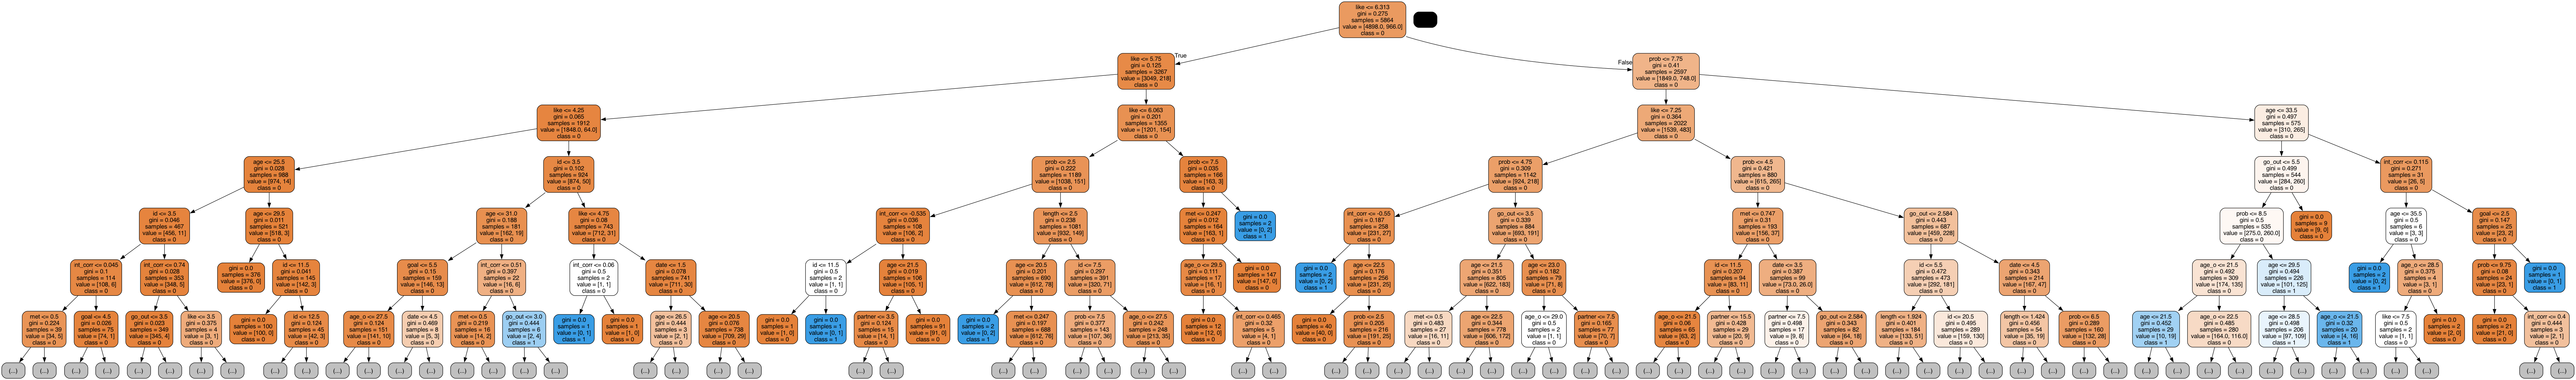
\includegraphics[width=\textwidth]{clf/holdout_tree_depth_6.png}\\[1em]
  
\includegraphics[width=\textwidth]{clf/cv_tree_depth_6.png}
  \caption{First 6 levels of the decision tree: top, trained in the holdout; bottom, trained on the last cross-validation fold.}
  \label{fig:arvores}
\end{figure}

\subsection{Additional experiments}

To understand the effect of some of the problems identified, we repeated the cross-validation (5 stratified folds) with a few variants. The results are in table~\ref{tab:extra}.

\begin{table}[H]
  \centering
  \small
  \begin{tabular}{lcccc}
    \toprule
     & Accuracy & Precision & Recall & F1 \\
    \midrule
    CART (baseline)                          & 0.765 & 0.307 & 0.341 & 0.323 \\
    CART, maximum depth 5                    & 0.836 & 0.512 & 0.091 & 0.154 \\
    CART, balanced class weights             & 0.778 & 0.326 & 0.324 & 0.325 \\
    CART, depth 5 and balanced weights       & 0.627 & 0.278 & 0.791 & 0.411 \\
    CART, without \code{id} and \code{partner} & 0.764 & 0.300 & 0.326 & 0.312 \\
    Naive Bayes (baseline)                   & 0.829 & 0.465 & 0.251 & 0.326 \\
    Naive Bayes, without \code{id} and \code{partner} & 0.828 & 0.457 & 0.249 & 0.322 \\
    \bottomrule
  \end{tabular}
  \caption{Additional experiments with 5-fold stratified cross-validation.}
  \label{tab:extra}
\end{table}

Removing the identifiers \code{id} and \code{partner} barely changes the results (F1 differences below 0.015). Limiting the tree depth to 5 raises accuracy to 0.84, but recall falls to 0.09, because the tree then almost always predicts class 0. Giving more weight to the minority class (\code{class\_weight='balanced'}) only has a clear effect when combined with the limited depth: recall rises to 0.79 and F1 to 0.41, the best value we obtained, but accuracy drops to 0.63 and precision to 0.28, i.e.\ the model predicts many matches that do not exist. This is a trade-off between false positives and false negatives, and the choice depends on the relative cost of each error.

\subsection{Critical discussion}

In terms of accuracy, Naive Bayes is better (about 0.82 to 0.83 against 0.76 to 0.77). This metric must be read with care: since 84\% of the examples belong to class 0, a classifier that always predicts 0 would have an accuracy of 0.84, higher than any of the four baseline models.

Precision measures, out of all predicted matches, how many really are matches, i.e.\ it penalises false positives. Naive Bayes is better (0.42 and 0.47 against 0.30 and 0.31): when it predicts a match it is right more often. Recall measures, out of all real matches, how many were found, i.e.\ it penalises false negatives. Here the tree is better (0.33 and 0.34 against 0.22 and 0.25): it finds more matches, at the cost of more false positives (table~\ref{tab:cm}). Naive Bayes is more conservative. F1 combines the two metrics and is low in all cases (0.29 to 0.33), which shows that neither model predicts the minority class well. Since the F1 values are close, we cannot say that one algorithm is clearly better overall.

Between the two evaluation strategies, cross-validation gives equal or higher values on every metric. The difference is small for the tree (about 0.01) and larger for Naive Bayes (about 0.04 in precision and 0.035 in F1). The holdout evaluates only 30\% of the data (2514 examples, 414 positives), so it is more sensitive to that particular test set. With a single run and without measuring variability, we cannot conclude that these differences are significant.

\subsection{Limitations and difficulties}
\label{sec:limitacoes}

\begin{itemize}
  \item \textbf{Class imbalance.} Only about 16\% of the examples are positive. The baseline models use no balancing technique, which hurts recall and F1. In the additional experiments we tested class weights, but not oversampling or undersampling.
  \item \textbf{Data size.} The data set has just over eight thousand examples and, in practice, many of them concern the same participants. With more data we would expect better predictions.
  \item \textbf{Identifier as attribute.} We used \code{id} (and \code{partner}) as attributes, although they are identifiers. They may introduce bias, because the same participant appears in several rows and the model may learn patterns specific to each person. In the additional experiments we found that removing them barely changes the results, but the final model should do without them.
  \item \textbf{Tree without complexity control.} In the baseline model we did not limit the depth or prune the tree (the depth reaches 27), so it overfits. We tested only one maximum depth (5), without choosing it by validation.
  \item \textbf{Evaluation.} Each experiment was run only once, with fixed seeds, so we did not measure the variability of the results. We also did not tune hyperparameters. In addition, the rows are not independent (the same participant appears in several rows). The data set has no unique participant identifier: \code{id} has only 22 distinct values, shared by participants from different events. As an approximation, we repeated the cross-validation grouping the rows by \code{id} (\code{StratifiedGroupKFold}), so that rows with the same \code{id} are either all in training or all in testing. F1 falls from 0.323 to 0.301 for the tree and from 0.326 to 0.316 for Naive Bayes (0.305 and 0.316 without \code{id} and \code{partner}), which suggests that plain cross-validation estimates are slightly optimistic. Since \code{id} is a coarse grouping, this difference is only an indication.
  \item \textbf{Difficulties.} The main difficulty was deciding how to handle missing values without losing too many rows, and realising that accuracy was a misleading metric for this problem. There were also practical difficulties with exporting the trees, which requires Graphviz to be installed on the system in addition to the Python library.
\end{itemize}

\clearpage
\section{Conclusions}

We compared Decision Trees (CART) and Gaussian Naive Bayes in predicting matches in speed dating events, using holdout and cross-validation. Naive Bayes has better accuracy (0.82 to 0.83 against 0.76 to 0.77) and better precision; the tree has better recall. F1 is low in all cases (0.29 to 0.33), because the positive class is a minority (about 16\%) and accuracy alone is misleading. Cross-validation gives equal or slightly better results than the holdout. In the additional experiments, combining class weights with a limited depth raised F1 to 0.41, with a loss of accuracy, and removing the identifiers had little effect. As future work, we propose choosing the hyperparameters by validation, testing other balancing techniques, using a unique participant identifier to group the cross-validation, and repeating the experiments with several seeds.

\begin{thebibliography}{9}
\bibitem{missing} \emph{A Comprehensive guide on handling Missing Values}. \url{https://medium.com/bycodegarage/a-comprehensive-guide-on-handling-missing-values-b1257a4866d1}\hfill\null
\bibitem{sklearn} Pedregosa \emph{et al.}, \emph{Scikit-learn: Machine Learning in Python}, Journal of Machine Learning Research, 12:2825--2830, 2011.
\bibitem{russell} S. Russell and P. Norvig, \emph{Artificial Intelligence: A Modern Approach}, Pearson, 4th ed., 2020.
\end{thebibliography}

\clearpage
\appendix
\section{Confusion matrices per fold}
\label{app:cm}

\begin{figure}[H]
  \centering
  \begin{subfigure}{0.4\textwidth}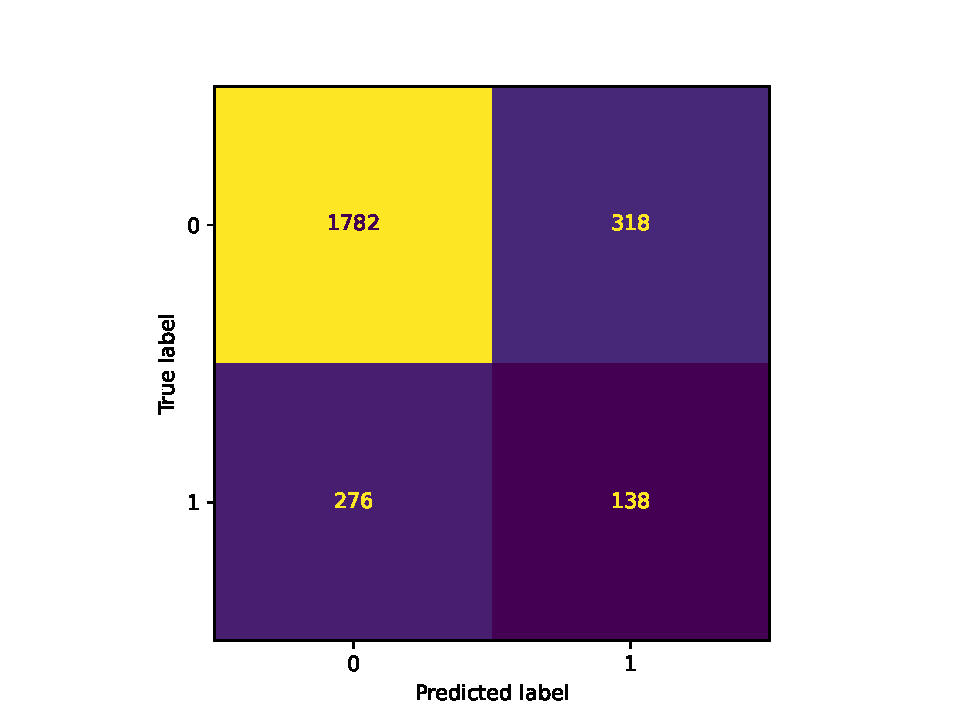
\includegraphics[width=\textwidth]{clf/holdout_confusion_matrix_.pdf}\caption{Holdout}\end{subfigure}
  \begin{subfigure}{0.4\textwidth}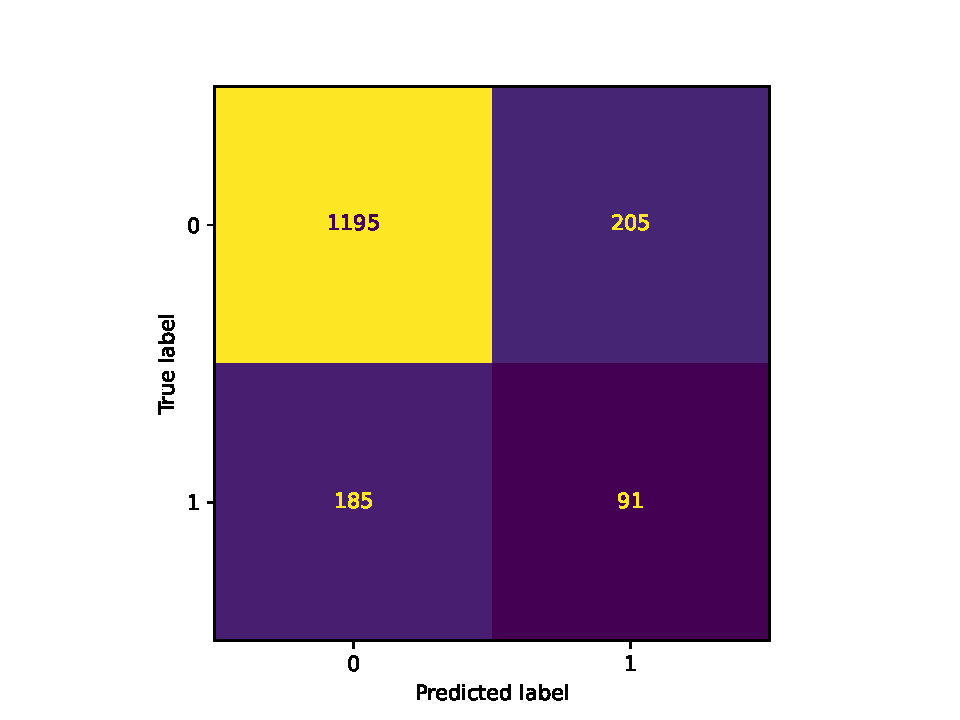
\includegraphics[width=\textwidth]{clf/cv_confusion_matrix_1.pdf}\caption{CV, fold 1}\end{subfigure}
  \begin{subfigure}{0.4\textwidth}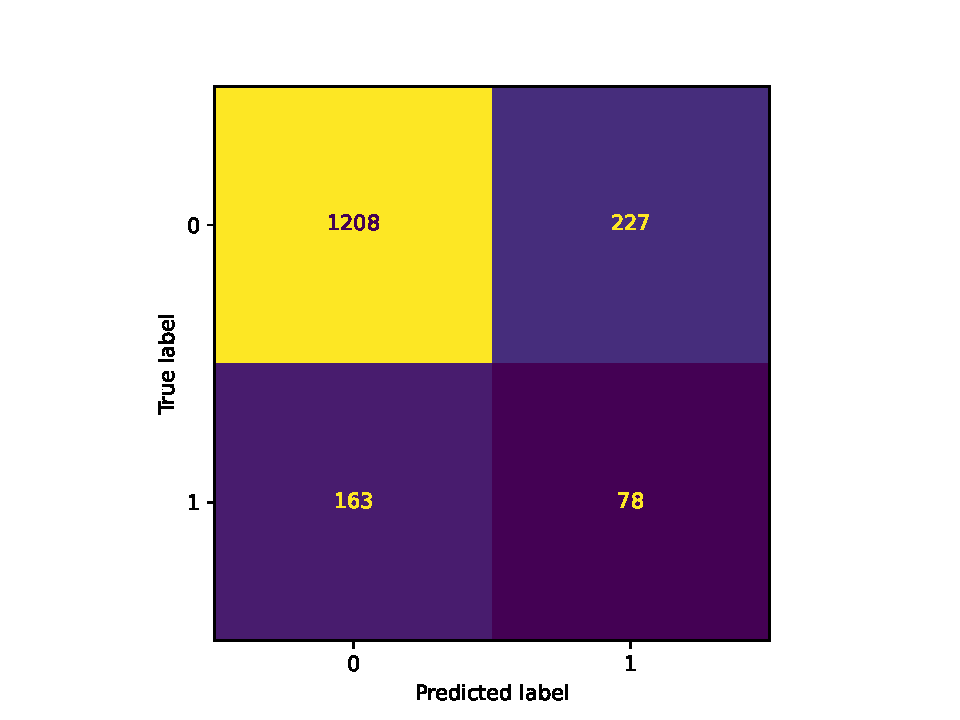
\includegraphics[width=\textwidth]{clf/cv_confusion_matrix_2.pdf}\caption{CV, fold 2}\end{subfigure}\\[0.5em]
  \begin{subfigure}{0.4\textwidth}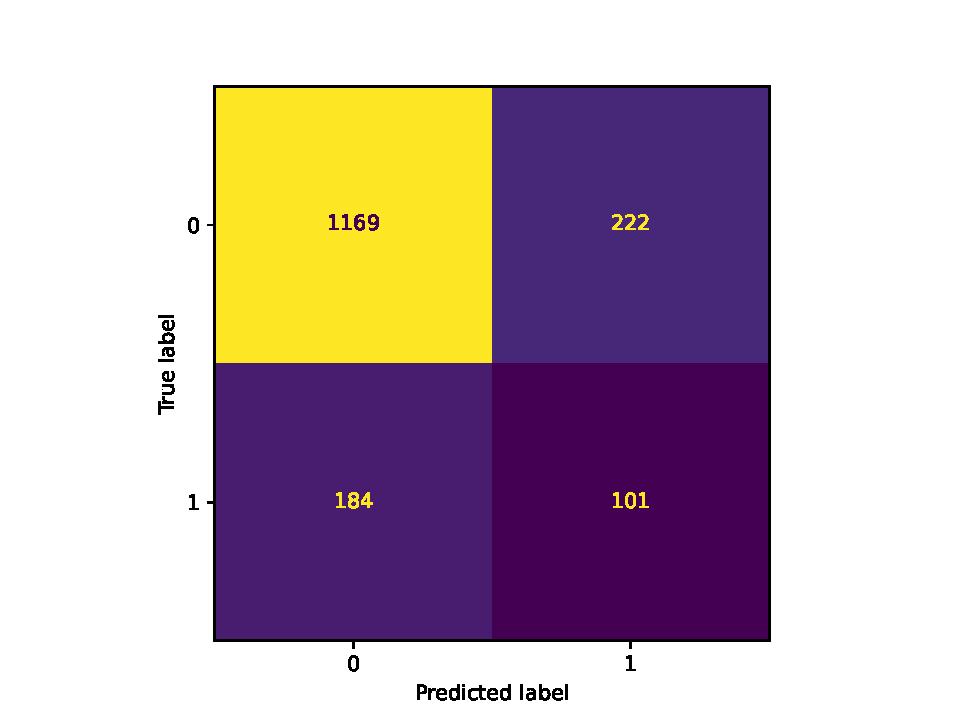
\includegraphics[width=\textwidth]{clf/cv_confusion_matrix_3.pdf}\caption{CV, fold 3}\end{subfigure}
  \begin{subfigure}{0.4\textwidth}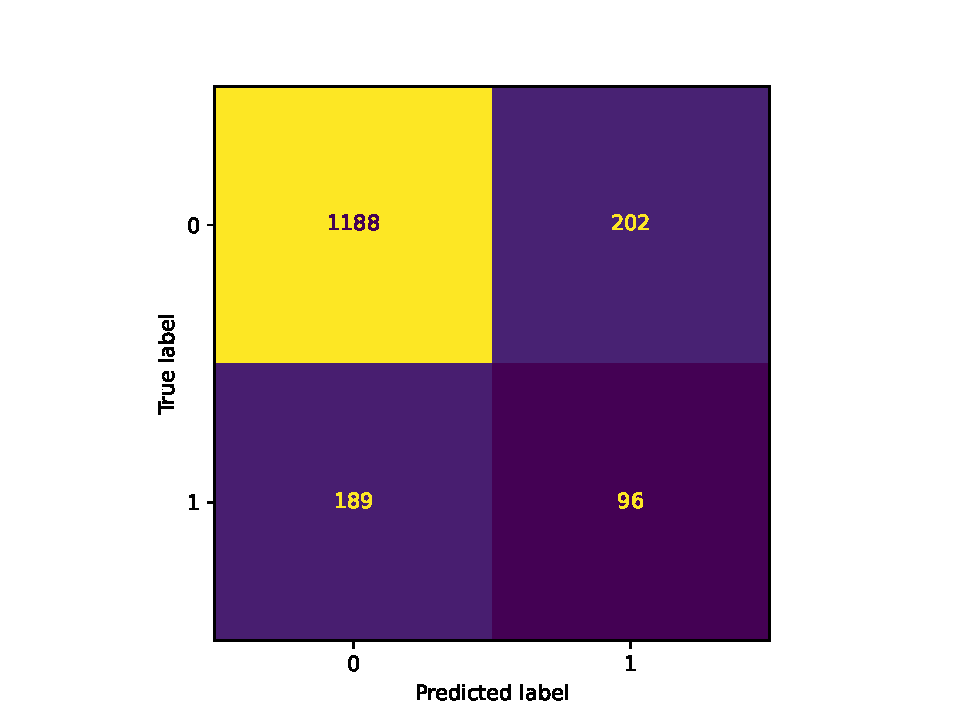
\includegraphics[width=\textwidth]{clf/cv_confusion_matrix_4.pdf}\caption{CV, fold 4}\end{subfigure}
  \begin{subfigure}{0.4\textwidth}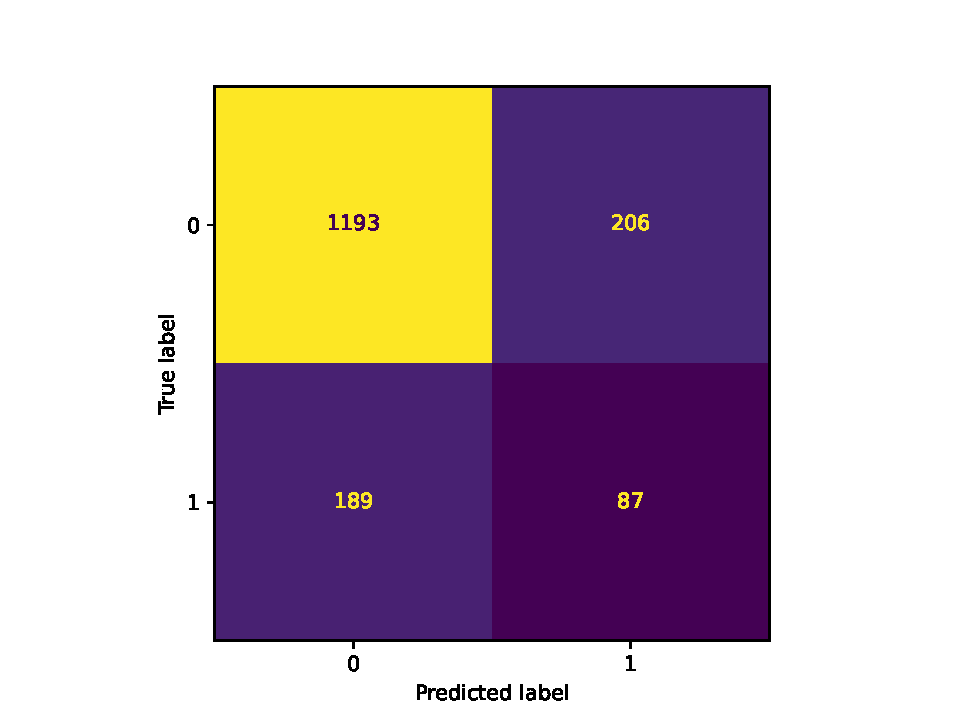
\includegraphics[width=\textwidth]{clf/cv_confusion_matrix_5.pdf}\caption{CV, fold 5}\end{subfigure}
  \caption{Confusion matrices of the decision tree (CART).}
  \label{fig:cart}
\end{figure}

\begin{figure}[H]
  \centering
  \begin{subfigure}{0.4\textwidth}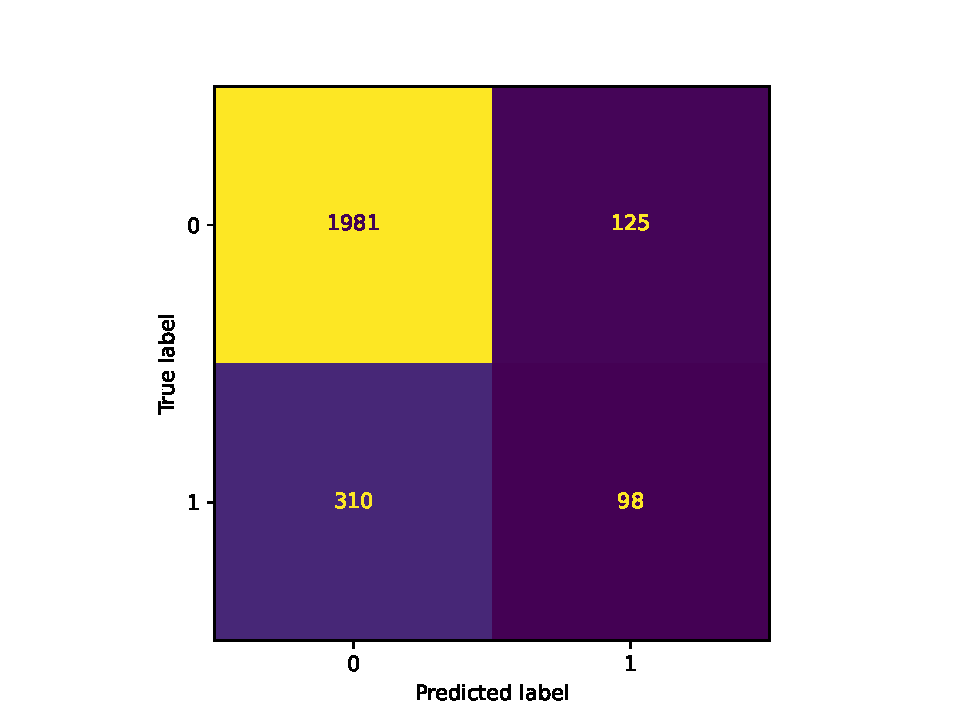
\includegraphics[width=\textwidth]{gnb/holdout_confusion_matrix_.pdf}\caption{Holdout}\end{subfigure}
  \begin{subfigure}{0.4\textwidth}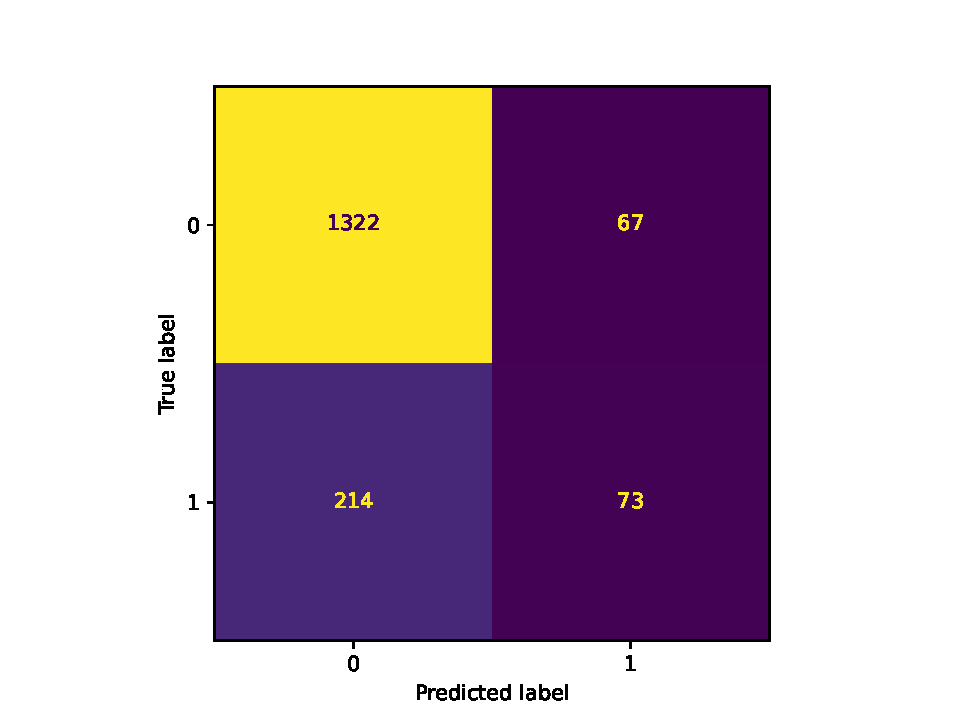
\includegraphics[width=\textwidth]{gnb/cv_confusion_matrix_1.pdf}\caption{CV, fold 1}\end{subfigure}
  \begin{subfigure}{0.4\textwidth}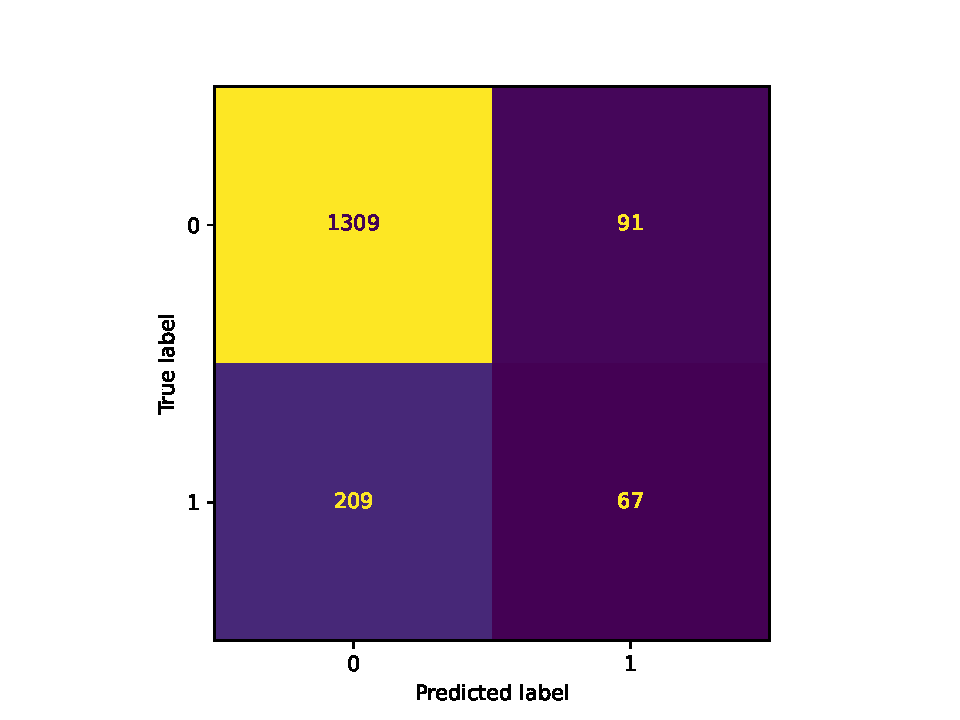
\includegraphics[width=\textwidth]{gnb/cv_confusion_matrix_2.pdf}\caption{CV, fold 2}\end{subfigure}\\[0.5em]
  \begin{subfigure}{0.4\textwidth}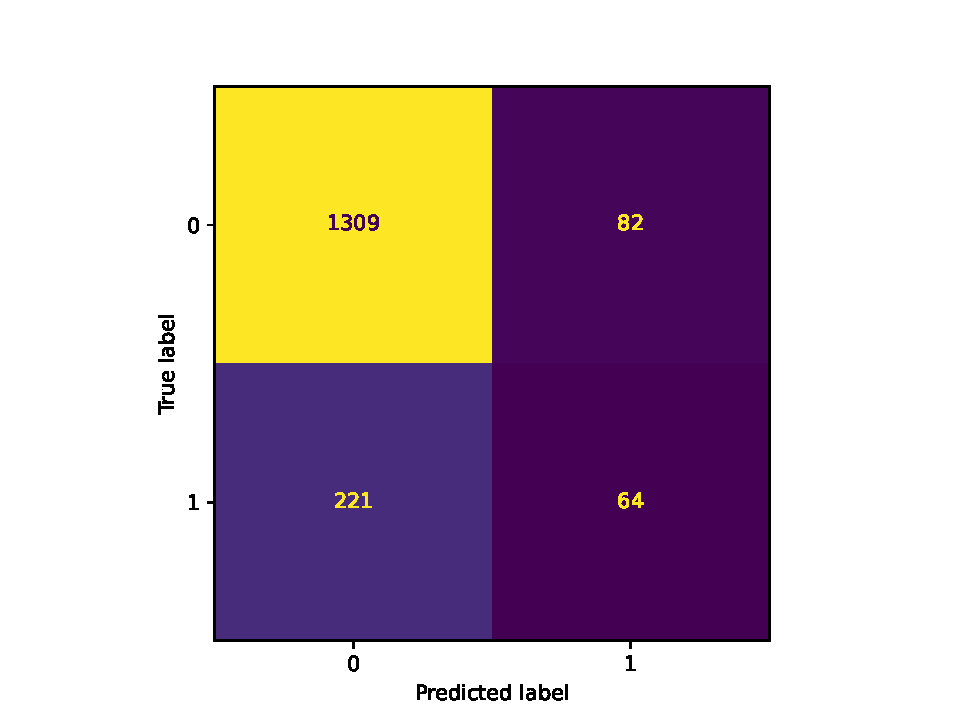
\includegraphics[width=\textwidth]{gnb/cv_confusion_matrix_3.pdf}\caption{CV, fold 3}\end{subfigure}
  \begin{subfigure}{0.4\textwidth}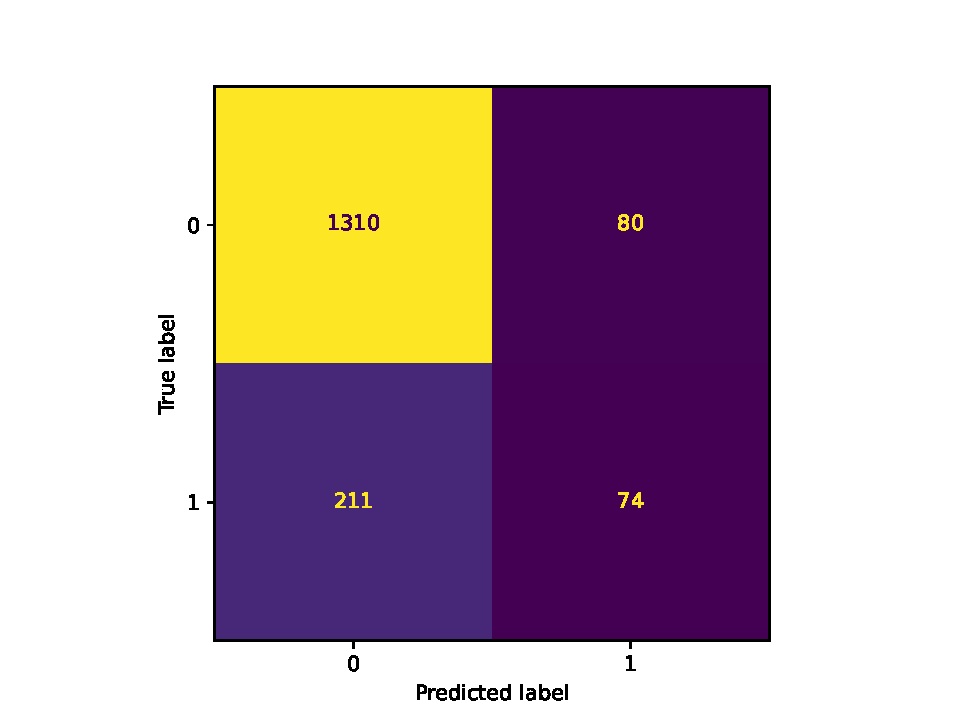
\includegraphics[width=\textwidth]{gnb/cv_confusion_matrix_4.pdf}\caption{CV, fold 4}\end{subfigure}
  \begin{subfigure}{0.4\textwidth}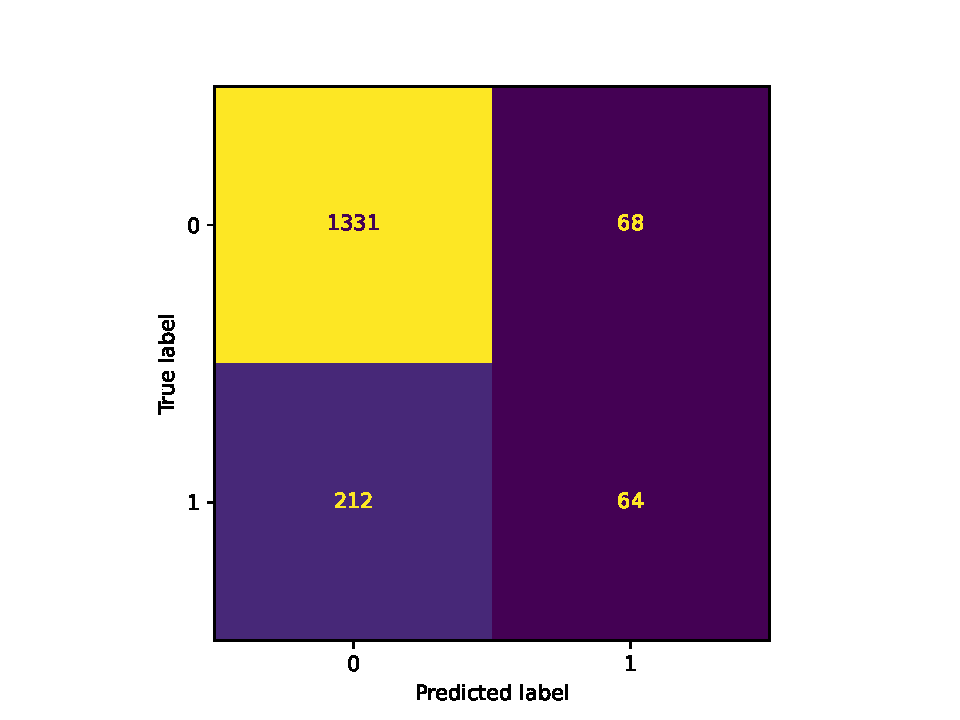
\includegraphics[width=\textwidth]{gnb/cv_confusion_matrix_5.pdf}\caption{CV, fold 5}\end{subfigure}
  \caption{Confusion matrices of Gaussian Naive Bayes.}
  \label{fig:gnb}
\end{figure}

\end{document}
